\section*{Abstract}
\label{sec:abstract}

The interaction of a user with an end device such as a smartphone or a computer is very diverse and difficult to predict. Nevertheless, user-specific (personalized) as well as global (collaborative) patterns can possibly be worked out with the help of preceding user interactions. These could be used to predict the intention of a user or a group of users. It is interesting to know to what level of detail these predictions can be made reliably.
By making use of the continous on-device data an attempt can be made to gain more insights in the user behavior or even forecast their next actions.

It suggests itself to implement this with the help of user interactions in sessions on Android devices. For this purpose, the Sequential UI Tree data of the device could be tracked, filtered and labeled and then trained with a machine learning model to find similar interaction sequences and then make predictions. These can then be very coarse, such as predicting the next app. Or they can be very detailed, e.g., determining the next user action, such as filling out a form field.

A concept will be developed on how a model for predicting user intent could be built and how it could be applied to the user session. To this end, possibilities for collecting and vectorizing sequential UI trees (e.g., from the Android Accessibility Service) will be discussed (e.g., via Recurrent Neural Network (\textit{RNN}) \cite{quadrana2017personalizing} \cite{bansal2022remembering} \cite{pietro2022recommendationSystems}, \textit{Seq2Seq} Model \cite{chollet2017seq2seq},
\textit{Screen2Vec} Model \cite{li2021screen2vec}, 
\textit{Intention2Text} \cite{yu2020understanding}, \textit{Html2Vec} \cite{wu2022distributed}), which are designed to predict the user intent. Here, privacy and feature pre-filtering in UI data plays an important role. After that, personalized as well as collaborative data can be used in a hybrid approach. This model should then be made available to the user in an Android app service and, depending on the level of detail, suggest upcoming apps or actions to the user at a suitable time. It should also be considered whether the user can contribute to the learning process and improve suggested actions through feedback (labeling).
The performance of the model can be measured, for example, by indicators such as the amount of training data and time spent on the learning process. The effectiveness can be evaluated by accuracy metrics in predicting, for example, app categories \cite{google2023appCategory} or complete test sequences via Rico \cite{deka2017rico} or ERICA \cite{deka2016erica}.

\begin{figure}
  \centering
  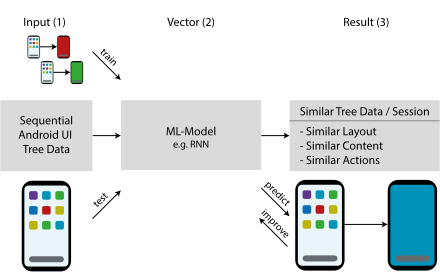
\includegraphics[width=\textwidth]{vectorization.svg}
  \caption{Possible procedure using a Machine-Learning algorithm to predict the next intent from a beginning user session: The input (1) can be a sequence of Android tree data. With help of a Machine-Learning-Model (2) (e.g. RNN) a vector representation can be trained and then predict the most probable action or screen (3) from a given starting sequence, but also can be improvde through the users feedback.}
  \label{fig:encode-decode}
\end{figure}

Furthermore, the machine learning model could provide the following benefits in addition to intent prediction:
\begin{itemize}
  \item reduction of the complexity and size of the UI tree
  \item creation of user groups that have similar behavior when using digital UI systems \cite{jayarajah2015need}
  \item elimination of technical expertise on individual features that would be required to manually compare user sessions \cite{ghods2019activity2vec}
  \item consideration of a user's history over time (sequential)
  \item comparison of user interactions without providing privacy invasive information
  \item supporting app developers to improve their app design and usability
  \item application in psychology and market research
  \item pre-loading of processes on devices (energy savings) \cite{shen2019deepapp}
\end{itemize}

As listed above, many fields of application can profit by elaborating such a system. It would be exciting to know, how the concrete concept would look like and if it can be implemented successfully e.g. to improve the user experience on end-user devices.

\begin{figure}
  \centering
  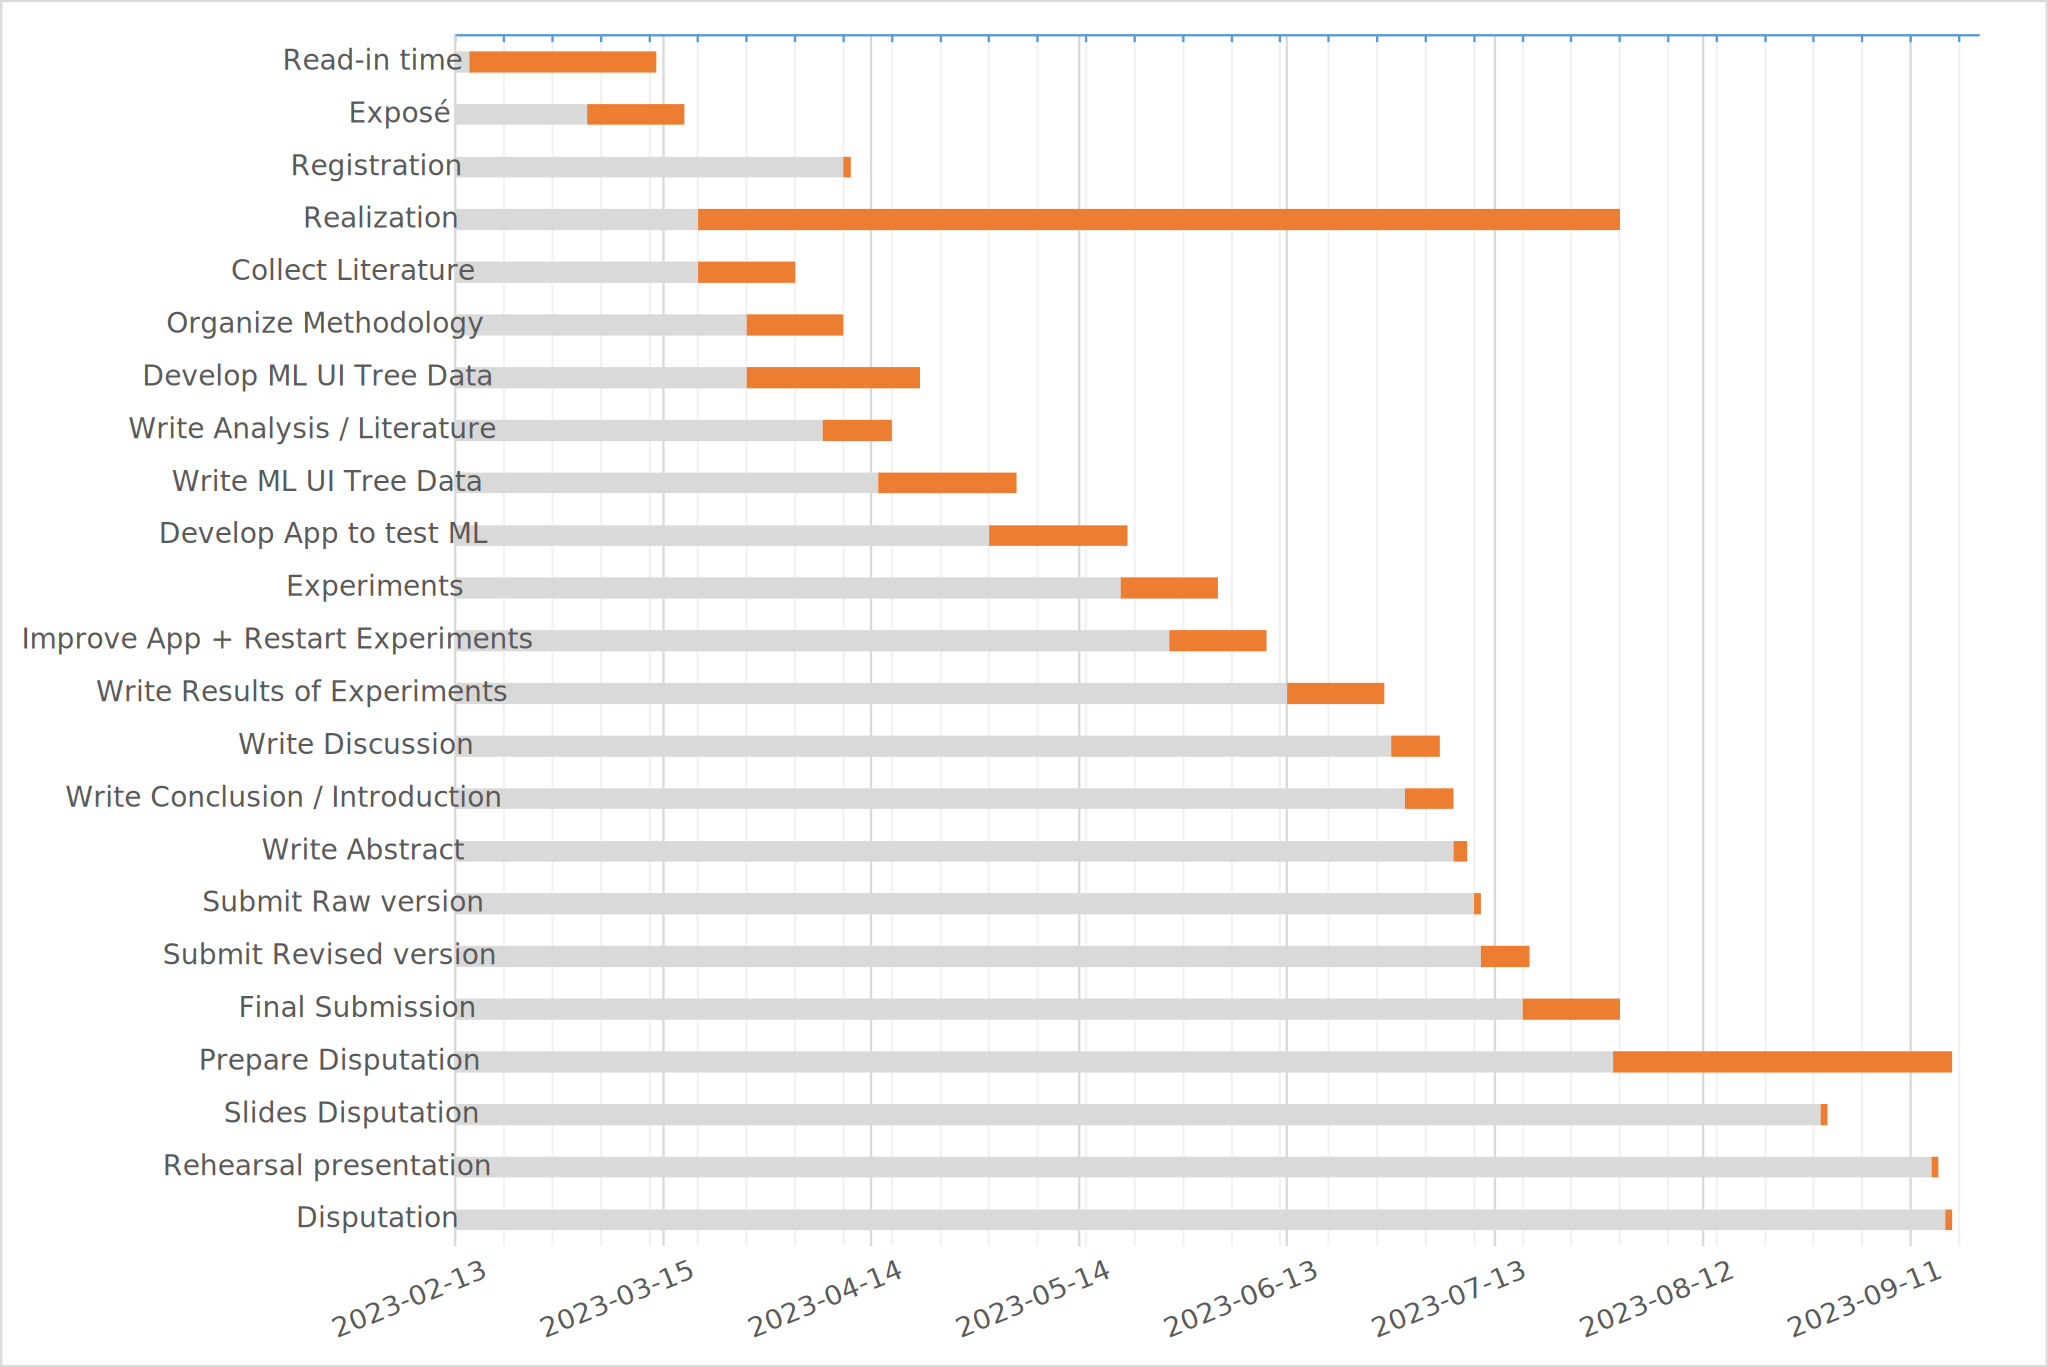
\includegraphics[width=\textwidth]{graphics/TimeTable-Gantt.svg}
  \caption{Schedule as a Gantt Chart}
  \label{fig:schedule}
\end{figure}